For the longitudinal controller, the closed loop block diagram including an integrator is shown in Figure~\ref{fig:hw_vtol_PID_root_locus_altitude}.
\begin{figure}[htbp]
   \centering
   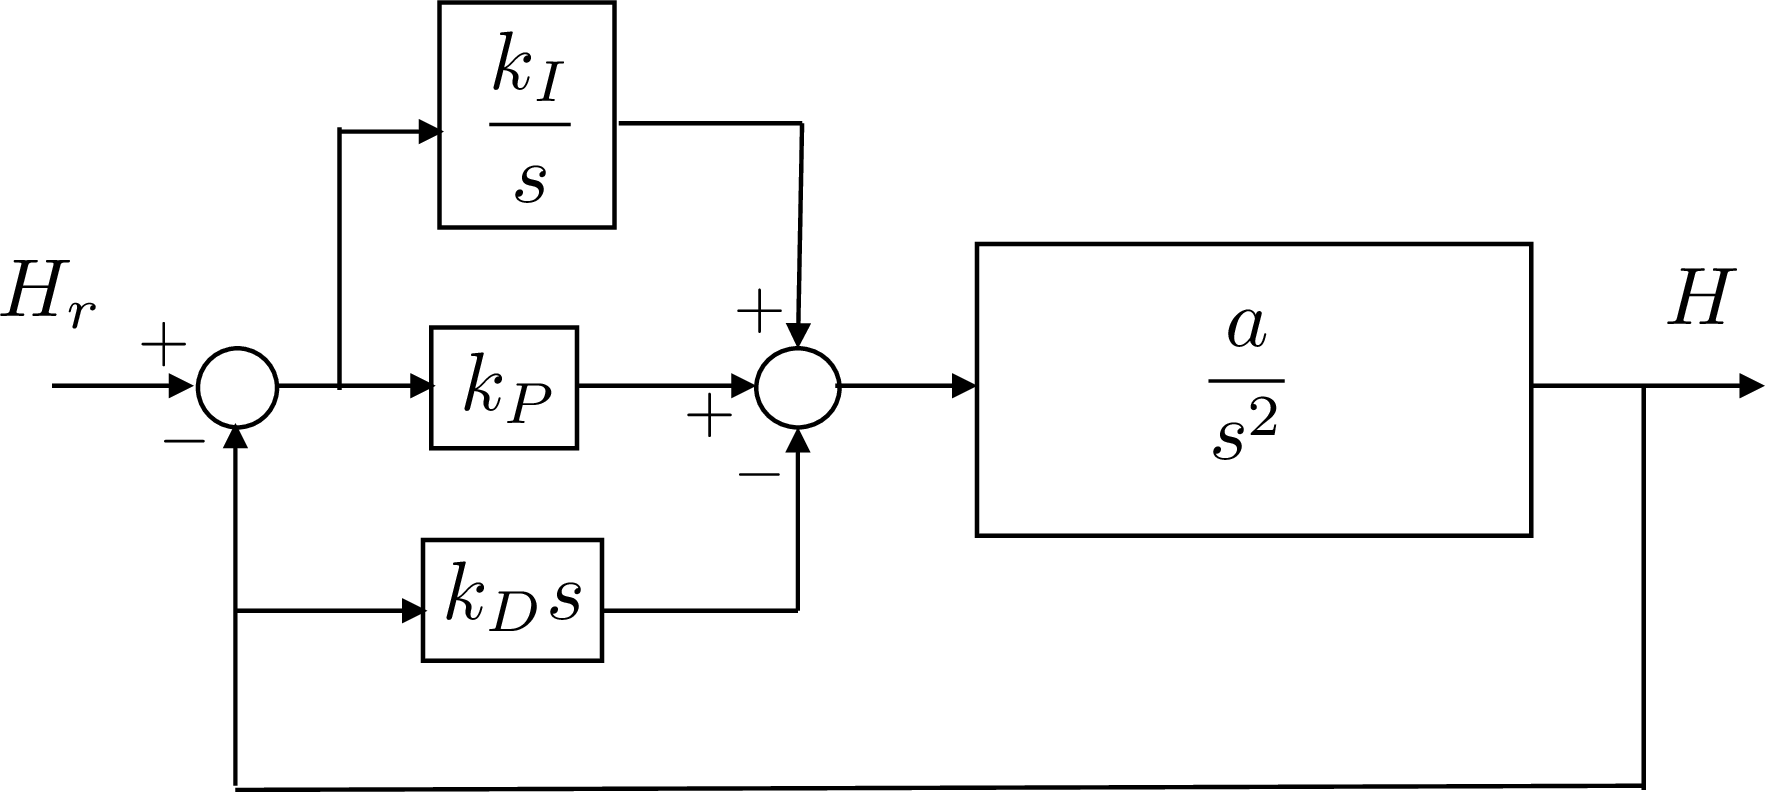
\includegraphics[width=0.6\textwidth]{6_design_studies/figures/hw_vtol_PID_root_locus_altitude.pdf}
   \caption{PID control for the longitudinal control of the VTOL system.}
   \label{fig:hw_vtol_PID_root_locus_altitude}
\end{figure}
The characteristic equation is given by
\[
1+P(s)C(s) = 1+\left(\frac{a}{s^2}\right)\left(\frac{k_Ds^2+k_Ps+k_I}{s}\right) = 0,
\]
where
\[
a = \frac{1}{m_c+2m_r}.
\]
Multiplying by the denominator and simplifying gives
\[
s^3+ak_Ds^2 + ak_Ps + ak_I = 0.
\]
Therefore, in Evan's form we have
\[
1 + k_I\left(\frac{a}{s^3 + ak_Ds^2 + ak_Ps}\right) = 0.
\]
The appropriate Matlab command is therefore
\begin{lstlisting}
>> L = tf([a],[1, a*kd, a*kp,0]);
>> figure(1), clf, rlocus(L);
\end{lstlisting}

For the outer loop of the lateral controller, the closed loop block diagram including an integrator is shown in Figure~\ref{fig:hw_vtol_PID_root_locus_lateral}.
\begin{figure}[htbp]
   \centering
   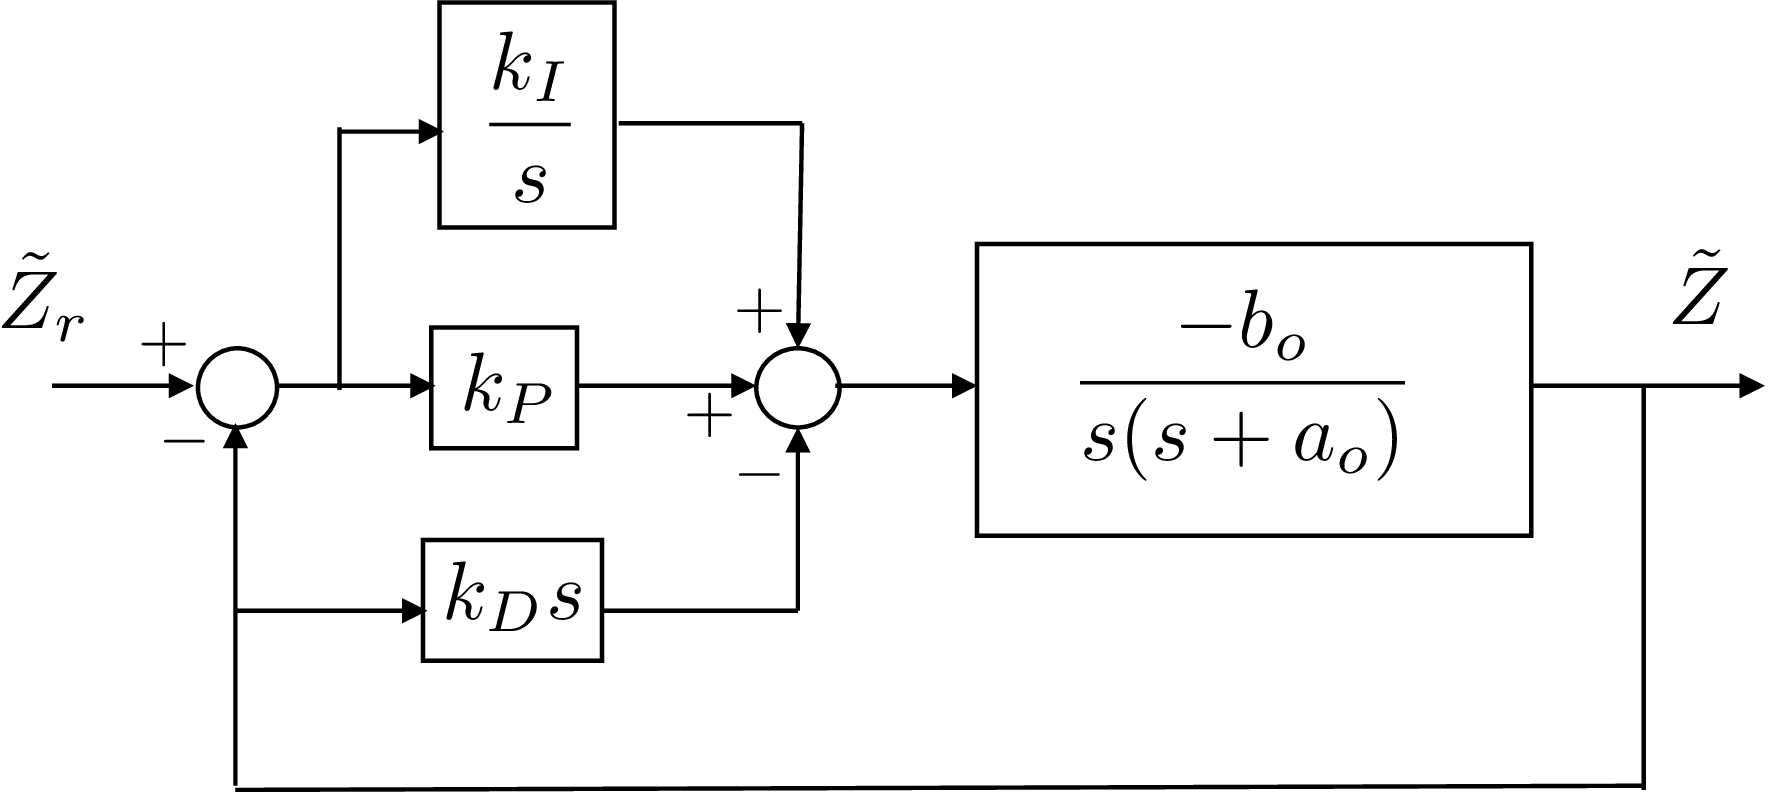
\includegraphics[width=0.6\textwidth]{6_design_studies/figures/hw_vtol_PID_root_locus_lateral.pdf}
   \caption{PID control for the outer loop of the lateral control of the VTOL system.}
   \label{fig:hw_vtol_PID_root_locus_lateral}
\end{figure}
The characteristic equation is given by
\[
1+P(s)C(s) = 1+\left(\frac{-b_o}{s(s+a_o)}\right)\left(\frac{k_Ds^2+k_Ps+k_I}{s}\right) = 0,
\]
where
\begin{align*}
a_o &= \frac{\mu}{m_c+2m_r} \\
b_o &= \frac{F_e}{m_c+2m_r}.
\end{align*}
Multiplying by the denominator and simplifying gives
\[
s^3+(a_o-b_ok_D)s^2 + (-b_ok_P)s + (-b_ok_I) = 0.
\]
Therefore, in Evan's form we have
\[
1 + k_I\left(\frac{-b_o}{s^3 + (a_o-b_ok_D)s^2 + (-b_ok_P)s}\right) = 0.
\]
The appropriate Matlab command is therefore
\begin{lstlisting}
>> L = tf([-bo],[1, (ao-bo*kd), -bo*kp,0]);
>> figure(1), clf, rlocus(L);
\end{lstlisting}
